\documentclass[a4paper,12pt]{article}
\usepackage[brazil]{babel}
\usepackage[utf8]{inputenc}
\usepackage[T1]{fontenc}
\usepackage{geometry}
\usepackage{setspace}
\usepackage{titlesec}
\usepackage{hyperref}
\usepackage{graphicx}
\usepackage{caption}
\usepackage{subcaption}
\usepackage{fancyhdr}
\usepackage{xcolor}

\input{commands.tex}

\hypersetup{
    colorlinks=true,% make the links colored
    linkcolor=blue
}

\usepackage{setspace}
\addbibresource{bibliography.bib}

\newcommand{\printingbibliography}{%

    \pagestyle{myheadings}
    \markright{}
    \sloppy
    \printbibliography[heading=bibintoc, % add to table of contents
                   title=Refer\^encias % Chapter name
                  ]
    \fussy%
}
\PassOptionsToPackage{table}{xcolor}
\renewcommand{\baselinestretch}{1.5}

\pagestyle{fancy}
\fancyhf{}
\renewcommand{\headrulewidth}{0pt}
\fancyhead[R]{\thepage}

\geometry{a4paper,top=30mm,bottom=20mm,left=30mm,right=20mm}

\titleformat*{\section}{\bfseries\large}
\titleformat*{\subsection}{\bfseries\normalsize}

\title{}
\author{Andr\'e V. Silva}
\date{\today}

\begin{document}
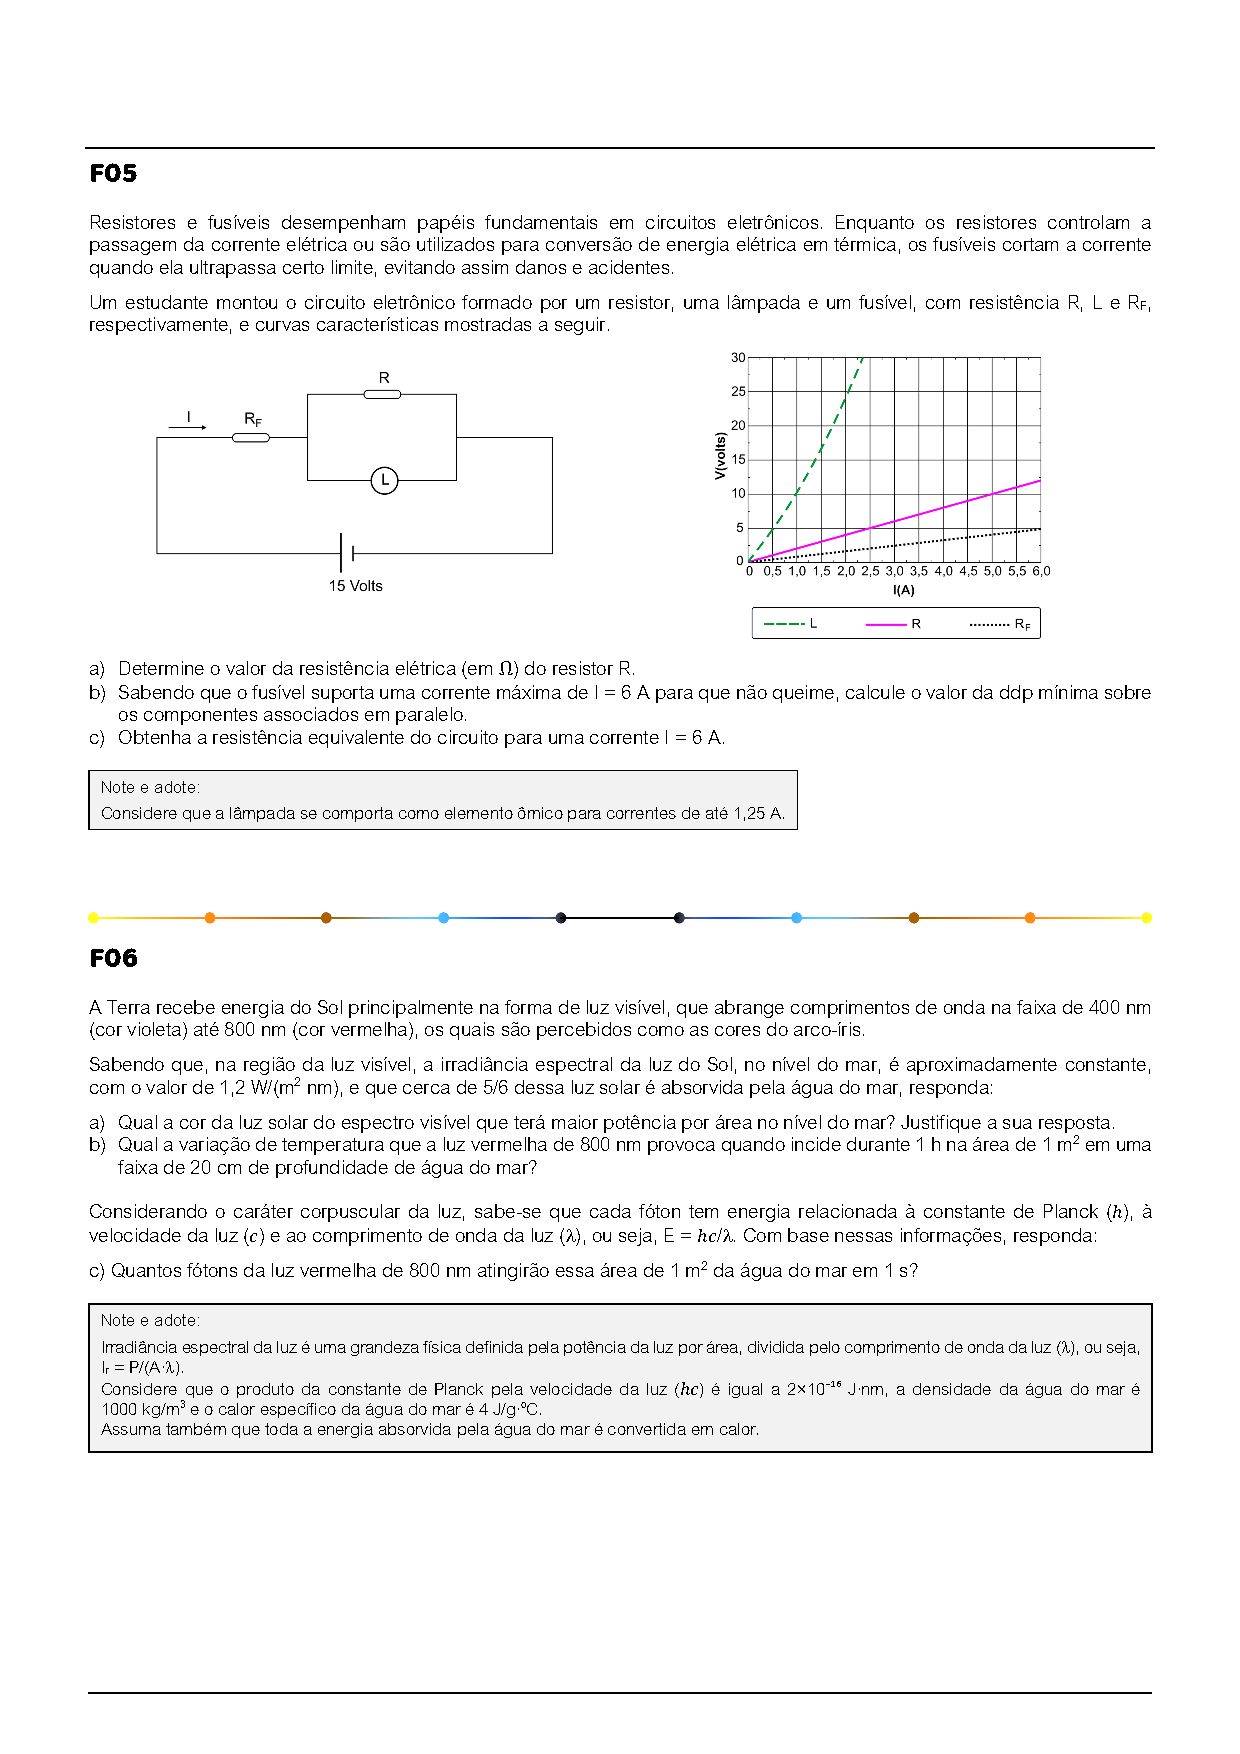
\includepdf[pages=-]{pg_0006.pdf}

\maketitle



\textbf{\textcolor{blue}{\Large Introdução Teórica}}\\

Em circuitos elétricos, os resistores são dispositivos que obedecem à \textbf{Lei de Ohm}, dada por:
\[
V = R\,I
\]
onde $V$ é a diferença de potencial, $R$ a resistência e $I$ a corrente elétrica.

Quando elementos estão em \textbf{paralelo}, todos possuem a mesma ddp, e a corrente total se divide entre eles:
\[
I = I_1 + I_2 + \cdots
\]

Já em \textbf{série}, a corrente é a mesma em todos os elementos e as tensões se somam:
\[
V = V_1 + V_2 + \cdots
\]

A resistência equivalente de resistores em paralelo é dada por:
\[
\frac{1}{R_{eq}} = \frac{1}{R_1} + \frac{1}{R_2}
\]

No gráfico $V \times I$, a inclinação da reta representa a resistência:
\[
R = \frac{V}{I}
\]

\textbf{Fusível:} atua como dispositivo de proteção, interrompendo o circuito quando a corrente ultrapassa um valor máximo.

\vspace{0.5cm}

\textbf{\textcolor{blue}{\Large Resolução}}\\

\textbf{a) Determinação da resistência $R$}

Pelo gráfico da curva do resistor (reta rosa), observamos um ponto:
\[
I = 6\,A \quad \text{e} \quad V = 12\,V
\]

Aplicando a Lei de Ohm:
\[
R = \frac{V}{I} = \frac{12}{6} = 2\,\Omega
\]

\textbf{Resposta:} $R = 2\,\Omega$

\vspace{0.5cm}

\textbf{b) ddp mínima nos elementos em paralelo}

O fusível suporta corrente máxima de $6\,A$. Para encontrar a ddp mínima, 
analisamos o comportamento do ramo em paralelo.

A lâmpada (L) é ôhmica até $1{,}25\,A$. 

Do gráfico, para $R_F$, temos:

\[
I = 6{,}0\,\text{A} \;\Rightarrow\; U_F = 5{,}0\,\text{V}
\]

Assim, para os elementos $R$ e $L$:
\[
U_R = U_L = U_{\text{total}} - U_F
\]
\[
U_R = U_L = 15\,\text{V} - 5{,}0\,\text{V}
\]

\[
\boxed{U_R = U_L = 10\,\text{V}}
\]


\vspace{0.5cm}

\textbf{c) Resistência equivalente do circuito para $I = 6\,A$}

Para $I = 6\,A$, usamos os valores do gráfico:

Resistor:
\[
R = 2\,\Omega
\]

Fusível:
\[
R_F = \frac{5}{6} \approx 0{,}83\,\Omega
\]

Lâmpada:
\[
R_L = 12\,\Omega
\]

Associação em paralelo (R e L):
\[
\frac{1}{R_{par}} = \frac{1}{2} + \frac{1}{12}
= \frac{6 + 1}{12} = \frac{7}{12}
\]

\[
R_{par} = \frac{12}{7} \approx 1{,}71\,\Omega
\]

Agora somamos com o fusível (em série):
\[
R_{eq} = R_F + R_{par}
\]

\[
R_{eq} = 0{,}83 + 1{,}71 = 2{,}54\,\Omega
\]

\textbf{Resposta:} $R_{eq} \approx 2{,}54\,\Omega$

\vspace{0.5cm}

\textbf{\textcolor{red}{Conclusão}}\\

\begin{itemize}
\item[(a)] $R = 2\,\Omega$
\item[(b)] $V_{mín} = 10\,V$
\item[(c)] $R_{eq} \approx 2{,}54\,\Omega$
\end{itemize}

\noindent\rule{\textwidth}{1pt}

\textbf{\textcolor{blue}{\Large Introdução Teórica}}\\

A radiação solar que atinge a Terra está majoritariamente na faixa da \textbf{luz visível}, compreendida entre comprimentos de onda de aproximadamente $400\,\text{nm}$ (violeta) a $800\,\text{nm}$ (vermelho).

A \textbf{irradiância espectral} $I_\lambda$ é definida como:
\[
I_\lambda = \frac{P}{A \cdot \Delta \lambda}
\]
onde $P$ é a potência incidente, $A$ a área e $\Delta \lambda$ a faixa de comprimento de onda.

Se a irradiância espectral é constante ao longo do espectro visível, então a potência por intervalo de comprimento de onda é uniforme.

\textbf{Energia do fóton:}
A energia de um fóton é dada por:
\[
E = \frac{hc}{\lambda}
\]
onde $h$ é a constante de Planck, $c$ é a velocidade da luz e $\lambda$ o comprimento de onda.

\textbf{Calor e variação de temperatura:}
A energia térmica absorvida por um corpo é:
\[
Q = m c \Delta T
\]
onde $m$ é a massa, $c$ o calor específico e $\Delta T$ a variação de temperatura.

\vspace{0.5cm}

\textbf{\textcolor{blue}{\Large Resolução}}\\

\textbf{a)} 
\[
I_r = \frac{P}{A \lambda} \;\;\Rightarrow\;\; \frac{P}{A} = I_r \cdot \lambda
\]

Com $I_r$ constante, $\dfrac{P}{A}$ é diretamente proporcional a $\lambda$. 

Isso significa que o valor máximo de $\dfrac{P}{A}$ estará associado ao valor máximo de $\lambda$, que corresponde à cor vermelha.

\vspace{0.4cm}

\textbf{b)} 

\textbf{(I)} A energia total $E_{\text{total}}$ recebida na superfície da água é obtida por:
\[
I_r = \frac{P}{A \lambda} \;\;\Rightarrow\;\; I_r = \frac{E_{\text{total}}}{\Delta t \cdot A \cdot \lambda}
\]

\[
1{,}2 = \frac{E_{\text{total}}}{3600 \cdot 1 \cdot 800}
\]

\[
\boxed{E_{\text{total}} = 3\,456\,000\ \text{J}}
\]

\vspace{0.3cm}

\textbf{(II)} A quantidade de calor sensível absorvida pela água é $Q$, tal que:
\[
Q = \frac{5}{6} E_{\text{total}} \;\;\Rightarrow\;\; Q = \frac{5}{6} \cdot 3\,456\,000
\]

\[
\boxed{Q = 2\,880\,000\ \text{J}}
\]

\vspace{0.3cm}

\textbf{(III)} Cálculo de $\Delta \theta$:

\[
Q = m \cdot c \cdot \Delta \theta \;\;\Rightarrow\;\; Q = d_{\text{água}} \cdot V \cdot c \cdot \Delta \theta
\]

\[
Q = d_{\text{água}} \cdot A \cdot h \cdot c \cdot \Delta \theta
\]

Com:
\[
Q = 2\,880\,000,\quad d_{\text{água}} = 1000\,\text{kg/m}^3,\quad A = 1\,\text{m}^2,\quad h = 0{,}20\,\text{m}
\]
\[
c = 4\,\frac{\text{J}}{\text{g}^\circ\text{C}} = 4 \times 10^3\,\frac{\text{J}}{\text{kg}^\circ\text{C}}
\]

\[
2\,880\,000 = 1000 \cdot 1 \cdot 0{,}20 \cdot 4 \times 10^3 \cdot \Delta \theta
\]

\[
\boxed{\Delta \theta = 3{,}6^\circ\text{C}}
\]

\section*{c) (I) Cálculo da energia de um fóton (quantum de energia)}

\[
E = \frac{hc}{\lambda}
\]

Sendo:
\[
hc = 2 \times 10^{-16} \ \text{J}\cdot\text{m}
\quad \text{e} \quad
\lambda_{\text{vermelha}} = 800 \ \text{nm}
\]

\[
E = \frac{2 \times 10^{-16}}{800} \ (\text{J}) 
\quad \Rightarrow \quad
E = 2{,}5 \times 10^{-19} \ \text{J}
\]

\vspace{0.5cm}

\section*{(II)}

Em 1h = 3600s $\longrightarrow$ 3 456 000 J

Em 1s $\longrightarrow e$

\[
e = 960 \ \text{J}
\]

\vspace{0.5cm}

\section*{(III)}

O número de fótons $N$ associado à energia $e$ fica determinado por:

\[
N = \frac{e}{E}
\quad \Rightarrow \quad
N = \frac{960}{2{,}5 \times 10^{-19}} \ (\text{fótons})
\]

\[
N = 3{,}84 \times 10^{21} \ \text{fótons}
\]

\vspace{0.5cm}

\section*{Respostas}

\begin{itemize}
\item[a)] Cor vermelha (a de maior comprimento de onda).
\item[b)] 3{,}6$^\circ$C
\item[c)] $3{,}84 \times 10^{21}$ fótons
\end{itemize}

%%%%%%%% Bibliography 
% Os comandos para incluir as referências bibliográficas
%\printingbibliography

\end{document}
